\documentclass{article}
\AtBeginDocument{
\heavyrulewidth=.08em
\lightrulewidth=.05em
\cmidrulewidth=.03em
\belowrulesep=.65ex
\belowbottomsep=0pt
\aboverulesep=.4ex
\abovetopsep=0pt
\cmidrulesep=\doublerulesep
\cmidrulekern=.5em
\defaultaddspace=.5em
}

\usepackage{graphicx}
\usepackage{physics}
\usepackage{float}
\usepackage[usenames,dvipsnames]{xcolor}
\usepackage{tikz,amsthm,comment}
%\usepackage[printwatermark]{xwatermark}
\usepackage[export]{adjustbox}
\usepackage[section]{placeins}
\usepackage[caption=false]{subfig}
\usepackage[percent]{overpic}



%% --- citations set up
%\bibpunct{[}{]}{,}{n}{}{}
%\bibliographystyle{plainnat}
\bibliographystyle{apsrev}
%\usepackage[hidelinks]{hyperref} %boxes hidden, remove hidelinks if boxes are desired.
%% ------------------


%\usepackage[export]{adjustbox}
%\renewcommand{\headrulewidth}{0pt}
%\cfoot{\textcolor{gray}{This is a working draft.}}
%\rhead{\thepage}
%\lhead{}

%% --- manual commands ---
\definecolor{ForestGreen}{HTML}{668000}
\definecolor{red1}{HTML}{FF4136}
\definecolor{green1}{HTML}{00802b}

\newcommand{\<}{\langle}
\renewcommand{\>}{\rangle}
\newcommand{\up}{\uparrow}
\newcommand{\dn}{\downarrow}

\newcommand{\tcite}{\textcolor{red1}{cite}}
\newcommand{\pdag}{{\phantom\dagger}}
\newcommand{\kong}[1]{\textcolor{blue}{Kong: #1}}
\newcommand{\feng}[1]{\textcolor{ForestGreen}{Feng: #1}}
\newcommand{\nandini}[1]{\textcolor{red1}{Nandini: #1}}
\newcommand{\todo}[1]{\textcolor{red}{TODO: #1}} % <--- remove before submission
\newcommand{\etal}{\emph{et al.}}



%%%%%%%%%%%%%%%%%%%%%%%%%%%%%%%%%%%%%%%%%%%%%%%%%%%
\usepackage{arxiv}
\usepackage[utf8]{inputenc} % allow utf-8 input
\usepackage[T1]{fontenc}    % use 8-bit T1 fonts
\usepackage{hyperref}       % hyperlinks
\usepackage{url}            % simple URL typesetting
\usepackage{booktabs}       % professional-quality tables
\usepackage{amsfonts}       % blackboard math symbols
\usepackage{nicefrac}       % compact symbols for 1/2, etc.
\usepackage{microtype}      % microtypography
\usepackage{lipsum}
\usepackage{amsmath,amsthm,amssymb}
\usepackage{listings}
\usepackage{bm}
\usepackage{bbm}
\usepackage{soul}
\usepackage{algorithm}
\usepackage{algorithmic}


% number
\newcommand{\N}{\mathbb{N}}
\newcommand{\Z}{\mathbb{Z}}
\newcommand{\F}{\mathcal{F}}
\newcommand{\R}{\mathbb{R}}
\newcommand{\xx}{\mathbf{x}}
\newcommand{\indicator}[1]{\mathbbm{1}[#1]}

% graph
\newcommand{\vertex}{\mathcal{V}}
\newcommand{\edge}{\mathcal{E}}
\newcommand{\graph}{\mathcal{G}}
\newcommand{\epair}[1]{\langle #1 \rangle}
\newcommand{\mb}[1]{\mathbf{#1}}
% in align
\newcommand{\aeq}{&=}
% sum and int and detivative
\newcommand{\msum}[2]{\sum_{#1}^{#2}}
\newcommand{\msumd}{\sum_{i=1}^{n}}
\newcommand{\msumone}[1]{\sum_{#1=1}^{n}}
\newcommand{\mint}[2]{\int_{#1}^{#2}}
\newcommand{\mintegral}[4]{\int_{#1}^{#2}#3 d #4}
\newcommand{\mprime}{^\prime}
% matrix method
\newcommand{\tsp}{^\top}
\newcommand{\inv}{^{-1}}
\newcommand{\mstar}{^{*}}
% distance
\newcommand{\ltwonorm}[1]{\Vert#1\Vert_2}
\newcommand{\lsquare}[1]{\Vert#1\Vert^2}
\newcommand{\lspace}[1]{\Vert#1\Vert }
\newcommand{\lone}[1]{\Vert#1\Vert_1}
% probability
\newcommand{\e}{\mathbb{E}} % Captical e
\newcommand{\cov}[2]{\mathbf{Cov}(#1,#2)}


% For STAT 203 Only
% Note: the sign for tilde is \sim
\newcommand{\asymeq}{\sim} % For asymptotic equivalence
%\newcommand{\so}[1]{o(#1)} % For small o
\newcommand{\bo}[1]{O(#1)} % For big O
\newcommand{\sameorder}{\asymp} % For same order
\newcommand{\conl}{\xrightarrow{\mathcal{L}}} % For convergence in law
\newcommand{\conp}{\xrightarrow{\mathcal{P}}} % For convergence in probability
\newcommand{\conr}{\xrightarrow{r}} % For convergence in rth mean
\newcommand{\conqm}{\xrightarrow{qm}} % For convergence in quadratic mean
\newcommand{\conas}{\xrightarrow{a.s.}} % For almost surely convergence 
\newcommand{\asngotoinfty}{$n\to\infty$} % For almost surely convergence
\newcommand{\ef}{\hat{f}_n}

% For this project only
\newcommand{\quest}[1]{\textcolor{red}{Question: #1}}
\newcommand{\answer}[1]{\textcolor{blue}{Answer: #1}}
\newcommand{\rx}[1]{\bm{x}_{#1}}
\newcommand{\rxi}{\bm{x}_{i}}
\newtheorem{theorem}{Theorem}[section]
\newtheorem{corollary}{Corollary}[theorem]
\newtheorem{lemma}[theorem]{Lemma}
\theoremstyle{definition}
\newtheorem{definition}{Definition}[section]
\newcounter{example}[section]
\newenvironment{example}[1][]{\refstepcounter{example}\par\medskip
   \noindent \textbf{Example~\theexample #1} \rmfamily}{\medskip}

\numberwithin{equation}{section}

\title{Markov Chain Monte Carlo:\\
From theory to method}


\author{
  Deqian Kong\thanks{This is a pedagogical paper on MCMC} \\
  Department of Statistics\\
  University of California, Los Angeles\\
  Los Angeles, CA 90095 \\
  \texttt{deqiankong@ucla.edu} \\
\
    \And
  Shi Feng$^*$ \\
  Department of Physics\\
  The Ohio State University\\
  Columbus, OH 43210 \\
  \texttt{feng.934@osu.edu} \\
  
  %% \AND
  %% Shi Feng \\
  %% Affiliation \\
  %% Address \\
  %% \texttt{email} \\
  %% \And
  %% Coauthor \\
  %% Affiliation \\
  %% Address \\
  %% \texttt{email} \\
  %% \And
  %% Coauthor \\
  %% Affiliation \\
  %% Address \\
  %% \texttt{email} \\
}


\begin{document}
\maketitle

\section{Introduction}
The essence of Markov Chain Monte Carlo (MCMC) method is to solve a problem by mapping it onto an iterative sampling problem of statistics, whereby the sampling procedure is governed by an engineered kernel so that the iteration converges to the result of the original problem. This is particularly useful when dealing with problems which have exponentially large searching space which makes them hard to solve by enumeration, or where there is a computational wall that is hard to penetrate by existing algorithms, like exactly diagonalizing a huge Hamiltonian.   

Although MCMC is widely used to simulate statistical ensembles (e.g. thermal average), the target of the original problem need not have statistical essence (e.g. Finding the ground state wavefunction of a Hamiltonian). In the latter case, iterations in MCMC serves as a statistical detour around the computational wall that stands between the destination and the starting point, and may be perceived as a useful intermediary redundancy which is ultimately to be removed by convergence at the fixed point.

\feng{add more examples in physics}



\bigskip

\textit{What does a physicist mean by \emph{sampling}?}

Statisticians and physicists use the word sampling not in exactly the same convention. In the view of a physicist (dummy physicist like Shi), sampling simply means imposing an observable operator (a Hermitian matrix) $\hat{O}$ on a system's Hilbert space for multiple times, which involves an average over either quantum or thermal ensemble, or both. In other words, given an observable $\hat{O}$, some information is inevitably coarse-grained by the sampling thus not detectable even though the statistical mechanics of the underlying microscopics are well-modeled. This perception is a top-down picture, whereby details of the system cannot be thoroughly pinned down as we stand at the top side, and the sampled data are perceived as shadows of true physical laws distorted and coarse-grained by probes. Such deficiency of physical sampling will always be with us, and every physicist has to learn to live with it. Nonetheless, as statisticians will tell us in MCMC, we sometimes can utilize this fact as our strengths to give predictions of physical properties with decent accuracy. 


\bigskip
\textit{What does a statistician mean by \emph{sampling}?}

A statistician will argue, as the resolution of our probe will never be enough to pin down every detail of the underlying mechanics, why not just coarse-grain the theory at the first place, thus calculations can be rendered easier. Hence, in statistics, sampling means the selection of a subset of all theoretical elements, or rather, distributions, to resemble the essence of the theory such that we can give a good enough prediction with lower cost. The simplest example will be the uniform random sampling.  


Suppose we want to evaluate the integral:
\begin{equation}
    J = \int f(x) p(x) dx 
\end{equation}
where $p(x)$ is a probability density distribution, $f(x)$ is some physical property that is dependent on microscopic states $x$. Naively all we need to do is evaluate the integral by brute force and get the number output. But instead of doing such a verbose calculation, a simpler way is to obtain
independent and \emph{evenly distributed} samples $\{x_1, x_2, \ldots, x_N\}$ from $p(x)$, and calculate
\begin{equation}
    J = \sum_i^N f(x_i) p(x_i) / N
\end{equation}
But the problem with this method is that the sampling resolution has to be extremely sharp when the density of states is huge somewhere. Hence if the theoretical distribution $p(x)$ is spiky at a few $x$, we have to make significantly more sample points in order to tackle those peaks, even though the rest of $p(x)$ are flat that doesn't cost much. There is another preferred way that addresses this problem, whereby samples are picked up in such a way that they resembles the key information of the continuous distribution $p(x)$, thus $J$ can be evaluated by
\begin{equation}
    J = \sum_i^N f(x_i) / N
\end{equation}
which should give a decent approximation of the original theory. In case of the canonical ensemble with Boltzmann distribution, the probability density $p(x) \propto \exp{-\beta E}$ has most of its weight close to $E = 0$, and a thin, long tail at higher $E$. Hence to do the aforesaid sampling, the subset of points that we need to pick up from $p(x)$ need to concentrate more at low energy and become sparse at high energy, so the essential information is captured. In MCMC, it is equivalent to
\begin{equation}
    J = \sum_{t=0}^N f(x_t) / N
\end{equation}
where each $x_t$ is a configuration sampled at time $t$ generated by some MCMC kernel, and it is expected to  converge to the true $J$ when $N$ is large enough. This is exactly what the pioneers of MCMC in physics community did in \cite{MetropolisPhys} where authors used such nonuniform sampling to calculate thermal averages in canonical ensembles. 







\section{Markov Chain  Basics}
In this section we introduce the generic routine of MCMC, that is, to find a iteration kernel $K$ that leads to the convergence to desired result, in which the final fixed point must satisfy the detailed balance condition (thus a global balance).   

The current state in a Markov chain only depends on the most recent previous states, i.e,
$$P(X_t|X_{t-1}.X_{t-2},\dots,X_0)=P(X_t|X_{t-1})$$
\begin{definition}[Markov Chain] 
$MC=(\Omega, \hat{v}_0, \hat{K})$, where $\Omega$ is the state space, $\hat{v}_0:\Omega\to\R$ is the initial probability distribution function over the states, $\hat{K}:\Omega\times\Omega\to\R$ is the transition probability function. Where the hats on $\hat{K}$ and $\hat{v}_0$ are used to emphasize they are essentially maps instead of numbers. 
\end{definition}

\textit{Remark: }In many places the Markov Chain are defined without hats as $MC=(\Omega, v_0, K)$. This may lead to the confusion in expression like $v_0 K$ as it is usually written. Because maps do not multiply, but only interact via composition i.e. $v_0\circ K$. Yet most of times $v_0 K$ are used to describe the probability distribution, which is a tuple of real numbers instead of a composite map. Therefore we use the hats to distinguish probability distribution from probability distribution function. In the forthcoming texts, we will denote the evaluated probability function by lower case letters. For example
\[
v_0 = \hat{v}_0 \cdot \Omega, \;\; \; K = \hat{K} \cdot (\Omega \times \Omega)
\]
where $v_0$ and $K$ can be perceived as real-valued vector and matrix.  Elements in vector $v_0$ are real-valued probability of all configurations $\omega_i \in \Omega$, and elements in matrix $K$ are conditional probabilities that connect pairs of configurations.   


\begin{example}
In the simplest Ising model on an $a \times b = N$ sites with $S_i = \pm 1$, the state space $\Omega$ is the collection of all configurations i.e. $\Omega =  \bigotimes^{N} \mathbb{Z}_2$, with the total number of states $\#\Omega = 2^{N}$. Each element $\omega \in \Omega$ is a $N$ dimensional tuple whose elements have value $\pm 1$. The initial probability distribution is denoted by the evaluated probability function $v_0$, a real-valued tuple, where the subscript $0$ says that the probability distribution is at zeroth iteration. Of course the initial probability distribution $v_0$ is arbitrary thus not the desired distribution which we are trying to sample. Our goal is then to find a way to evolve $v_0$ to $v_1, \ldots, v_n$, hoping such a series would ultimately converge to the true probability distribution, e.g. the Boltzmann weights $e^{-\beta E_{\omega}}$ for the Ising model in a canonical ensemble. This evolution of probability distribution is described by the aforementioned $K$.
\end{example}






At time $n$, the Markov Chain state will follow a probability for finite states, and the state converge to an invariant probability,
\[v_n=v_0K^n \text{ and }\lim_{n\to\infty}v_0K^n=\pi\] 
Our objective is to design a Markov chain kernel $K$, such that $\pi$ is the unique, invariant probability of $K$ (a fixed point). Suppose we are given $\Omega$ and a target probability $\pi = (\pi_1,\cdots ,\pi_N)_{(1\times N)}$, our goal is to design $v_0$ and $K$ so that $\pi K=\pi$, which is a necessary condition.

Here we check the conditions for topology of transition matrix:
\begin{itemize}
  \item stochastic matrix: $\sum_{j=1}^NK_{ij}=1,\forall i \in \Omega, K_{ij}\ge 0$ or $K\bm{1}_{N\times 1}=\bm{1}$
  \item global balance: $\pi_{1\times N} K=\pi$, $\sum_{i=1}^N\pi_iK_{ij}=\pi_j,\forall j \in \Omega$
  \item detailed balance(\textit{reversible}): $\pi_iK_{ij}=\pi_jK_{ji},\forall i,j\in\Omega$

  We should know that the detailed balance is a sufficient but not necessary condition for global balance and we should know detailed balance indicates stationarity and in particular global balance,
  \[\pi K=\msumd \pi_i[K_{i1},\cdots,K_{iN}]=\msumd [\pi_1K_{1i},\cdots,\pi_NK_{Ni}]=\pi\]
  \[\sum_{i=1}^N\pi_iK_{ij}=\pi_j\sum_{i=1}^NK_{ji}=\pi_j\]
  \item irreducibility: A Markov Chain is irreducible if its transition matrix $K$ has only one communication class. $i\to j$, denotes a state $j$ is accessible from $i$, if there exists a finite step $M$, such that \[K^M_{ij}=\sum_{i_1,i_2,\cdots,i_{M-1}}K_{ii_1}K_{i_1i_2}\cdots K_{i_{M-2}i_{M-1}}K_{i_{M-1}j}>0\]
  $i\leftrightarrow j$ generates a partition of the state space into disjoint equivalence(communication) classes given by $\Omega=\cup^C_{i=1}\Omega_i$ and one communication class means all the states are accessible from each other
  \item Aperiodicity: to define this, we need to define a periodic MC first. An irreducible MC with transition matrix $K$ has period $d$ if there is a unique patition of graph $G$ into cyclic classes:
  \[C_1,C_2\cdots,C_d,\sum_{j\in C_k}K_{ij}=1,\forall i\in C_{k-1}\]
  In an periodic Markov Chain there is no connection between states within each individual cyclic class, 
  and an irreducible Markov chain with transition matrix $K$ is aperiodic if it’s largest period is $d = 1$.
  \item stationarity distribution: A Markov chain with transition kernel $K$ has stationary distribution $\pi$ if\[\pi K=\pi\]
  There may be many stationary distributions w.r.t $K$. Even if there is a stationary distribution, a Markov chain may not always converge to it.
\end{itemize}

\begin{theorem}[Perron-Frobenius*]
For any primitive (irreducible and aperiodic) $N\times N$ stochastic matrix $K$, with eigenvalues
\[\lambda_1>|\lambda_2|>\cdots>|\lambda_r|\] and multiplicities as $m_1,m_2,\cdots,m_r$, with $\bm{u}_1=\pi,\bm{v}_1=\bm{1}$ has the biggest eigenvalue $\lambda=1$ with $m_1=1$.
\end{theorem}
Proofs can be found \href{http://people.math.harvard.edu/~knill/teaching/math19b_2011/handouts/lecture34.pdf}{here} in both numerical($tr(K)=\msumd K_{ii}=\msum{i=1}{r}m_i\lambda_i$) and geometric perspective(by defining sphere $x_1^2+x_1^2+\cdots+x_n^2=1$). More detailed one can be found \href{http://pi.math.cornell.edu/~web6720/Perron-Frobenius_Hannah\%20Cairns.pdf}{here}.

For a square matrix, we have eigen decomposition as $K=Q\Lambda Q\inv$ and as \asngotoinfty,
\[K^n=Q\Lambda Q\inv=Q\Lambda^n Q\inv\to \lambda_1\bm{v}_1\bm{u}_1=\bm{1}\pi\]



\subsection{A worked example of balance equations}
The global balance equations are a set of equations that characterize the (dynamical) equilibrium distribution (or any stationary distribution, for example, a composite chemical system in a dynamical equilibrium). 

Suppose at time $t$ we have some initial pdf configuration $\pi^{(0)} = (p_1, p_2)$ which may be perceived as a discrete pdf of two distinct chemical compounds, and the transition matrix $K$ is defined:
\[
	K=
\begin{pmatrix}
	k_{11} & k_{12} \\ k_{21} & k_{22}
\end{pmatrix}
.\] 
that is, at time $t+1$ the new distribution $\pi'$ is:
\begin{equation}
	\pi^{(1)} = \pi^{(0)} K = 
	\begin{pmatrix}
		p_1 & p_2
	\end{pmatrix}
	\begin{pmatrix}
	k_{11} & k_{12} \\ k_{21} & k_{22}	
	\end{pmatrix}
	= (p_1 k_{11} + p_2 k_{21},\; p_1 k_{12} + p_2 k_{22})
\end{equation}
with the row-major index notation we can write:
\begin{equation}
	\pi_i^{(1)} = \sum_{j} \pi_j^{(0)} k_{ji},\;\;\;\;\text{with } i,j \in \{1,2\}
\end{equation}
If the system reaches an equilibrium state at time $T$, then the state at next moment $T+1$ should remain the same (to be precise, they are element-wise the same), that is:
\begin{equation}
	 \pi_i^{(T+1)} = \sum_{j} \pi_j^{(T)} k_{jk} = \pi_i^{(T)}
\end{equation}
For short, we say at equilibrium we have a fixed point characterized by
\begin{equation}
	\boxed{\pi_i = \sum_{j} \pi_j k_{ji} }
\end{equation}
In the context of probability theory, let $\Omega$ be the total state space, and let $\mathbf{a}, \mathbf{b} \in \Omega$ be two different states. Suppose at time $t$ the probability for the system to stay in state $\mathbf{a}$ is $p(\mathbf{a})$, and the probability of state $\mathbf{a}$ to transit into state $\mathbf{b}$ at next moment $t+1$ is $p(\mathbf{a}_t \rightarrow \mathbf{b}_{t+1})$. Therefore, the probability for the system to stay in state $\mathbf{b}$ at $t+1$ and in $\mathbf{a}$ at the previous moment is:
\begin{equation}
	p(\mathbf{b}_{t+1}, \mathbf{a}_t) = p(\mathbf{a}_t) p(\mathbf{a}_{t} \rightarrow \mathbf{b}_{t+1})
\end{equation}
note that we have implicitly used that  $p(\mathbf{a} \rightarrow \mathbf{b})$ is essentially a conditional distribution i.e. $p_t(\mathbf{a} \rightarrow \mathbf{b})	\equiv p_t(\mathbf{b}_{t+1}|\mathbf{a}_t)$. Now note that not only can $\mathbf{a}$ transit to $\mathbf{b}$, but there can be many other states which have non-zero probability to transit into $\mathbf{b}$ in the next moment. Therefore, the probability of the system to stay in state $\mathbf{b}$ is 
\begin{equation}
	p(\mathbf{b}_{t+1}) = \sum_{n} p(\mathbf{b}_{t+1}, \mathbf{n}_t) = \sum_{n} p(\mathbf{n}_t)p(\mathbf{n}_t \rightarrow \mathbf{b}_{t+1})  
\end{equation}
Now we can identify $p(\mathbf{b}_{t+1})$ as $v_b^{(t+1)}$: the probability that the system be at $b-$th state at the $t+1$, and $p(\mathbf{a}_t \rightarrow \mathbf{b}_{t+1})$ as $k_{ab}$: the probability that the system transits from $a$-th state at $t$ to $b$-th state at $t+1$:
\[
    p(\mathbf{b}_{t+1})\;\;\; \iff \;\;\;v_b^{(t+1)}
\]
\[
    p(\mathbf{a}_t \rightarrow \mathbf{b}_{t+1})\;\;\; \iff \;\;\;k_{ab}
\]
Therefore the global interation can be written as:
\begin{equation}
	v_b^{(t+1)} = \sum_{j} v_a^{(t)} k_{ab} 
\end{equation}
or in the matrix form:
\begin{equation}
	\mathbf{v}^{(t+1)} = \mathbf{v}^{(t)} \mathbf{K}
\end{equation}
if the a fixed poin is reached at $T$ then:
\begin{equation}
	\mathbf{v}^{(T)} = \mathbf{v}^{(T+1)} = \mathbf{v}^{(T)}\mathbf{K} 
\end{equation}




\section{Statistical Error Analysis and Binning}
Note: MCMC samples are correlated. Discuss the independent case, then discuss the correlated case. Error bar can be crucial in Baysian mothods. Call central limit theorem. 

\section{The Metropolis-Hastings Algorithm}
% \quest{what exactly are iterating? In the formalism it seem we are evolving probability $v_0,\ldots,v_n$ by $K$ i.e. it is the map $v: \Omega \rightarrow \mathbb{R}$ that iterates and converges to $\pi$. But in Ising model we are evolving the configuration $\vec{x}_1, \ldots, \vec{x}_n \in \Omega$, instead of the map $v_0, \ldots, v_n: \Omega \ni \vec{x} \mapsto \mathbb{R}$.}

% \answer{To be formal, $v_i$ is a map from the whole possible state space $\Omega$ to $\R$, which is a distribution function $f(\cdot)$ with definition domain $\Omega$ and value domain $\R$ \textcolor{red}{I think it's better Not to call it a distribution. A distribution is a tuple of real numbers, but a map here is essentially a \textit{diagram} that connects some math objects to real numbers. I explain this in the new Q\&A sections}. But in practice, it can be $\R^n$ in n-dim case. The key here is that $v_i$ maps from state space to real valued domain. In the previous notation, we are trying to evolve $v_0$ to $v_n$ to make it close to $\pi$. While in the case of Ising model, we need to clearly make connections between "configuration" and "map" as you mentioned. In 1-d Ising case, we have $x_1,x_2,\cdots,x_n\in\{0,1\}$ \textcolor{red}{I think dimension is not relevant here, this is true for arbitrary dimension, like any n-d matrix is equivalent to a ordered 1d tuple}. "Configuration" here denotes one choice of $\{x_i,i=1,2\cdots,n\}\in \{0,1\}^n$, which is exactly a distribution function mapping from state space to real valued domain, $\R^n$ here. In short, maps = distribution function = configuration \textcolor{red}{maps are not configurations, same problem explained in new Q\&As}.\\
% However, you might confuse with the energy function we used in Gibbs sampler when we iterate. It's a technique that helps us iterates across all possible states. When computing the detailed balance, we only care about the distribution function in each consecutive state.\\
% M-H algorithm and Gibbs sampler are two useful techniques that belong to MCMC because we can prove detailed balance respectively.}


% \quest{How can we multiply maps at all? When maps interact, they should not be connected by multiplication, but by composition (you don't multiply diagrams) e.g. $f\circ g$ instead of $f\times g$. So does $v_j K_{ji}$ means $v_j \circ K_{ji}$ or $v_j \times K_{ji}$?}

% \answer{I think there is a confusion in the notation. Essentially because maps cannot bE multiplied like real numbers, for maps are not real numbers. Hence in a way the notation $v_j\times K_{ji}$ doesn't make sense to me if they are maps. Let us clarify the formalism in the following way: we have a map which we call probability map $v: \Omega \rightarrow \mathbb{R}$, and I like to point out this is not a real number even though it maps $\omega \in \Omega$ to a real number. In contrast, $v_i$ should NOT be viewed as a map in our relevant context. To be formally clear, $v_i$ is an \emph{implemented map} by $\omega_i\in\Omega$, that is, $v_i$ is NOT literally a map anymore, but a real number that is produced from $\omega_i$ by the map $v$ i.e.  $v_i = v(\omega_i)$. In the same way, $K$ is NOT real-valued conditional probabilities, but only a map $K:\Omega\times\Omega \rightarrow \mathbb{R}$ which cannot be multiplied. What we mean by $K_{ji}$ that can be multiplied is actually $K_{ji} = K(\omega_j, \omega_i)$. Therefore, $v_j K_{ji}$ is not multiplication nor composition of two maps, but multiplication of real numbers $v(\omega_j) K(\omega_j, \omega_i)$.   }


% \textcolor{blue}{In retrospect, the crux in my first question, where I can't distinguish iteration of configuration from that of map, is that I confused the following two: (1) the probability map $v:\Omega \rightarrow \mathbb{R}$ and (2) the implemented map on a configuration $\vec{\omega}_i \in \Omega$ in the ensemble, viz. \st{$v_i: \Omega \ni \vec{\omega}_i \mapsto \mathbb{R}$} which I perceived was wrong, it should be what I mentioned as $v_i = v(\omega_i)$. These real numbers $v_i$ are thereafter put into the ordered tuple denoted by $\mathbf{v}$, which provides a global description of the probabilities (discrete probability distribution) of all $\omega \in \Omega$ in an ordered way. We may clarify this by saying $\mathbf{v} = (v_i, \ldots, v_N) = (v(\omega_i), \ldots, v(\omega_N)) \in \mathbb{R}^N$. Hence to avoid confusion of notation conventions, we may refrain from using the word \emph{function} or \emph{map} arbitrarily, e.g. we don't multiply distribution functions, we only multiply distributions; we want iterations to converge to desired probability distribution $\pi$, not probability distribution function $\pi$, nor the map $\pi$. }

% \textcolor{blue}{
% I think it's also worth pointing out that the abstract map $v: \Omega \rightarrow \mathbb{R}$ itself is not important in our context. Since, in a practical scheme like MCMC, we do not (and cannot) evolve the map in any abstract sense, but rather we evolve it in terms of its representation $v_i = v(\omega_i),\; \forall \omega_i \in \Omega$, that is, a representative table supported on $\Omega$.  
% }

% \textcolor{blue}{
% \st{In the case of Ising model, we evolve the exceedingly simple distribution $v_i \in \mathbb{Z}_2$ with $\mathbb{Z}_2 \subset \mathbb{R}$. Note by $v_i \in \mathbb{Z}_2$ we mean we have chosen the basis of $\Omega$ by the occupation number $\{0,1\}$ (or whatever binary representation of $\mathbb{Z}_2$) on each pixel, instead of any fancy  patterns or collective modes. In conclusion, in Ising's MCMC, we do evolve the distribution, which is an alias for configuration (but it's not map in the abstract sense).} This is terribly WRONG! Let's tease out the correct intuition by Q\&A that follows. 
% }



% \quest{What role does $K(x,y)$ play in the generation of these samples. How does the global balance engage in the process.}

% \answer{The most confusing question to S. Feng the dummy is how do we iterate the $v_j^{(t)} K_{ji}$ when $v_j^{(t)}$ is an arbitrary intermediate distribution that is not even represented explicitly, or do we really iterate the distribution at all where it is  the configuration $x$ that evolves in practice.  }

% \textcolor{blue}{
% To articulate the answer, first of all there are several points worth noting: (1) The goal is to produce a set of samples $\{x_i\}$, not distributions $\{v_i^{(t)}\}$. (2) If the sampled points are too few, there is a large ensemble of possible $\mathbf{v}^{(t)}$s. (3) The scope of the ensemble decrease as we make samples using $K$, and shrinks (converges) to $\pi$ if we use $K$ by $N \rightarrow \infty$ times.   
% }

% \textcolor{blue}{
% So the question now is how to perceive the connection between the restriction on the ensemble and the generation of samples by $K$. Yes, someone has to tell me this....
% }





\begin{algorithm}
\caption{The Metropolis-Hastings Algorithm}
\label{algo:MH}
    \textbf{Input:} Target probability distribution $\pi(x)$, current state $x^{(t)}\in\Omega$, and the proposal probability distribution $Q(x,y)$.
    \textbf{Output:} New state $x^{(t+1)}\in\Omega$.\\
    1. Propose a new state y by sampling from $Q(x^{(t)},y)$.\\
    2. Compute the acceptance probability:
    \[\alpha(x,y)=\min\Bigg(1,\frac{Q(y,x)}{Q(x,y)}\cdot\frac{\pi(y)}{\pi(x)}\Bigg)\]
    3. With the probability $\alpha(x,y)$, we have $x^{(t+1)}=y$, otherwise $x^{(t+1)}=x^{(t)}$
\end{algorithm}
% Suppose the target probability distribution $\pi(x)$, current state $x^{(t)}\in\Omega$, and proposal probability distribution Q(x,y), new state $x^{(t+1)}\in\Omega$, we first propose a new state by sampling $Q(x^{(t)},y)$, then calculate the acceptance probability as

% with acceptance probability $\alpha(x,y)$, accept the move and make $x^{(t+1)}=y$, otherwise $x^{(t+1)}=x^{(t)}$.



As the above notations, for $x,y \in \Omega$, we have
\[ K(x,y) = \begin{cases} 
      Q(x,y)\alpha(x,y)=Q(x,y)\min\Bigg(1,\frac{Q(y,x)}{Q(x,y)}\cdot\frac{\pi(y)}{\pi(x)}\Bigg) & \textit{if } y\neq x\\
      1-\sum_{y\neq x}Q(x,y)\alpha(x,y) &\textit{if } y=x \\
   \end{cases}
\]
Next we want to prove this definition of transition matrix $K$ satisfies the detailed balance.
\begin{align*}
\pi(x)K(x,y)\aeq \pi(x)Q(x,y)\min\Bigg(1,\frac{Q(y,x)}{Q(x,y)}\cdot\frac{\pi(y)}{\pi(x)}\Bigg)=\min\Bigg(\pi(x)Q(x,y),\pi(y)Q(y,x)\Bigg)\\
\pi(y)K(y,x)\aeq \pi(y)Q(y,x)\min\Bigg(1,\frac{Q(x,y)}{Q(y,x)}\cdot\frac{\pi(x)}{\pi(y)}\Bigg)=\min\Bigg(\pi(y)Q(y,x),\pi(x)Q(x,y)\Bigg)
\end{align*}
In many cases, the target distribution is written as a Gibbs distribution or Boltzmann distribution,
\[\pi(x)=\frac{1}{Z}e^{-E(x)},\;\;\text{or}\;\;\pi(x)=\frac{1}{Z}e^{-E(x)/T}\]
For simplicity let us used Gibbs for an example. While the normalizing constant is hard to compute, suppose the proposal probability is symmetric, i.e. $Q(x,y)=Q(y,x)$, then the acceptance probability becomes
\[\alpha(x,y)=\min(1,\frac{\pi(x)}{\pi(y)})=\min(1,e^{-(E(x)-E(y))})=\min(1,e^{-\triangle E})\]
In this way, if $\triangle E<0$, i.e. state $y$ has lower energy, $\alpha(x,y)=1$, and $x^{(t+1)}=y$; if $\triangle E>0$, i.e. state $x$ has lower energy, $\alpha(x,y)=e^{-\triangle E}$. Note that $\triangle E$ is often computed locally as the two states $x$ and $y$ share most of their elements.

There exist other designs for the acceptance rate that guarantee the detailed balance equation, such as
\[\alpha(x,y)=\frac{\pi(y)Q(y,x)}{\pi(x)Q(x,y)+\pi(y)Q(y,x)}\]
Or more generally,
\[\alpha(x,y)=\frac{s(x,y)}{\pi(x)Q(x,y)}\]
where $s(x,y)$ is a symmetric function.

With this method, we can maximize a function for optimization by slowly changing the stationary distribution $\pi(x)$ with additional temperature $T$. The temperature starts from a high $T_0$ and decreased to 0 as \asngotoinfty.
\[\pi(x, T_n)=\frac{1}{Z(T_n)}e^{-E(x)/T_n}\]
which is known as simulated annealing method.


\subsection{Application of M-H method in Ising model}
The first implementation of M-H algorithm is carried out in 

\cite{MetropolisPhys}, 
whose underlying theory was given much later in \cite{Hastings}. 

See example C++ code in \href{https://github.com/fengshi96/MCMC}{https://github.com/fengshi96/MCMC}.




















\section{Gibbs Sampler}
Gibbs sampler was created for obtaining samples from distributions that are difficult to sample. Here we use the vector form, and $E(\xx)$ denotes the energy function,
\[\pi(\mathbf{x})=\frac{1}{Z}e^{-E(\xx)},\xx=(x_1,x_2,\cdots,x_d)\in\Omega\]

The Gibbs sampler was introduced as a stochastic version of the relaxation algorithm. In this way, we first introduce the relaxation algorithm, which has no no guarantees for finding the global optimum and in fact, it often gets stuck in local optima.
\begin{algorithm}
\caption{Relaxation Algorithm}
\label{algo:relaxation}
    \textbf{Input:}Energy function $E[\xx]$, current state $\xx^{(t)}=\{x_1,x_2,\cdots,x_d\}\in\Omega$ and each $x_i$ can have $L$ possible values as $\{y_1,y_2,\cdots,y_L\}$.\\
    \textbf{Output:} New state $\xx^{(t+1)}\in\Omega$.\\
    1. Select an index variable $i\in\{1,2,\cdots,d\}$ at random.\\
    2. Compute 
    \[u=\arg\min_{y_l}\Bigg(E(x_i=y_l|\xx_{-i})\Bigg)\textit{ for }l=1,2,\cdots,L\]
    3. Let
    \[\xx^{(t+1)}_{-i}=\xx^{(t)}_{-i} \text{ and } x^{(t+1)}_{i}=u\]
\end{algorithm}


In formal, the goal of Gibbs sampler is to sample a joint probability,
\[\xx=(x_1,x_2,\cdots,x_d)\sim \pi(x_1,x_2,\cdots,x_d)\]
by sampling in each dimension according to the conditional probability,
\[x_i\sim\pi(x_i|\xx_{-i})=\frac{1}{Z}\exp(-E(x_i|\xx_{-i}))\]
% Using the same notation as above, the procedure of Gibbs sampler is that after we select a variable $i\in\{1,2,\cdots,d\}$ with total $L$ values as $\{y_1,y_2,\cdots,y_L\}$ at random, computer the conditional probability vector $\mathbf{u}=(u_1,u_2,\cdots,u_L)$ with each element,
% \[u_l=\pi(x_i=y_l|\xx_{-i})\]
% Sample $j\sim\mathbf{u}$ and set $\xx^{(t+1)}_{-i}=\xx^{(t)}_{-i}$ and $x^{(t+1)}_{i}=y_j$.

\begin{algorithm}
\caption{Gibbs Sampler}
\label{algo:gibbs}
    \textbf{Input:}Target Probability function $\pi[\xx]$, current state $\xx^{(t)}=\{x_1,x_2,\cdots,x_d\}\in\Omega$ and each $x_i$ can have $L$ possible values as $\{y_1,y_2,\cdots,y_L\}$.\\
    \textbf{Output:} New state $\xx^{(t+1)}\in\Omega$.\\
    1. Select an index variable $i\in\{1,2,\cdots,d\}$ at random.\\
    2. Compute conditional probability vector $\mathbf{u}=(u_1,u_2,\cdots,u_L)$with 
    \[u_l=\pi(x_i=y_l|\xx_{-i})\]
    3. Sample $j\sim\mathbf{u}$ and set $\xx^{(t+1)}_{-i}=\xx^{(t)}_{-i}$ and $x^{(t+1)}_{i}=y_j$.
\end{algorithm}

Here I want to point out the difference explicitly. When updating one element of the current sample, relaxation algorithm finds the current local minimum and Gibbs sampler samples from its distribution. We should know that only find the local minimum will limit the stochasticity.

A \textit{sweep} of the Gibbs sampler is a sequential visit to all of the sites (variables) once.
Although the transition matrix $K_ii$ for one Gibbs step may not be irreducible and aperiodic, it is easy to show that the total transition matrix $K = K_1K_2\cdots K_d$ does have these features after one sweep. 

If we have $\xx^{(t)}\sim\pi(\xx)$, by above procedure,
\begin{align*}
\xx^{(t)}\aeq(x_1,\cdots,x_i,x_{i+1},\cdots,x_d)\sim \pi(\xx)\\
\xx^{(t+1)}&\sim\pi(y_j|\xx_{-i})\pi(\xx_{-i})\\
&\sim\pi(y_j|x_1,\cdots,x_{i-1},x_{i+1},\cdots,x_d)\pi(x_1,\cdots,x_{i-1},x_{i+1},\cdots,x_d)\\
\xx^{(t+1)}\aeq \pi(x_1,\cdots,x_{i-1},y_j,x_{i+1},\cdots,x_d)\sim \pi(\xx)
\end{align*}

\section{Cluster Sampling}
Let $\mathcal{G}=(\mathcal{V},\mathcal{E})$ be an adjacency graph. Each vertex $v_i\in\vertex$ has a state variable $x_i$ with a finite number of labels, i.e. $x_i\in\{1,2,\cdots,L\}$. If $\mb{X} = (x_1,x_2,\cdots,x_{|\vertex|})$ denotes the labeling of the graph, the Ising ($L=2$) or Potts ($L\ge3$) model is a Markov Random Field,
\[\pi(\xx)=\frac{1}{Z}\exp\Bigg({-\sum_{\epair{s,t}\in\edge}}\beta_{st}\indicator{x_s\neq x_t}\Bigg)\]
The Swendsen-Wang (SW) algorithm introduces a set of random variables on the edges indicating if they are connected or not,
\[\mathbf{U}=\Bigg\{\mu_e:\mu_e\in\{0,1\},\forall e\in\edge\Bigg\}\]
The edge is connected is $\mu_e=1$. The binary variable $\mu_e$
follows a Bernoulli distribution conditional on the labels of the vertices $e$ connects, $x_s$ , $x_t$,
\[\mu_e|(x_s,x_t)\sim Bernoulli\Bigg((1-e^{-\beta_{st}})\indicator{x_s=x_t}\Bigg),\forall e\in\edge\] 
$\mu_e=1$ with probability $1-e^{-\beta_{st}}$ if $x_s=x_t$ and $\mu_e=0$ with probability $1$ if $x_s\neq x_t$. 

The SW algorithm iterates the clustering and flipping step. In clustering step,
given the current labeling, we calculate the adjacency of the graph and form a set of connected components with the same label. In flipping step, we randomly select a connected component and assign an arbitrary color to all the lattice inside the connected component.
In this step, one may choose to perform the random color flipping for some or all of the connected components in $\mb{CP}$ independently, as they are decoupled. By doing so, all possible labelings of the graph are connected in one step, just like one sweep of the Gibbs sampler.


\begin{algorithm}[h]
\caption{Swendsen-Wang Algorithm}
\label{algo:sw}
    \textbf{Initialize:} The adjacency graph $\mathcal{G}=(\mathcal{V},\mathcal{E})$, a set of random variables for each edge as $\mathbf{U}=\{\mu_e:\mu_e\in\{0,1\} ,\forall e\in\edge\}$ denoting their connectivity and a set of random variables denoting the label of the lattice as $\mathbf{X}=\{x_i:x_i\in\{1,2,\cdots,L\},\forall i\in\vertex\}$.\\
    \textbf{Input:} Current connectivity of edges  $\mathbf{U}^{(t)}$ and labeling of lattice $\mathbf{X}^{(t)}$ at time $t$\\
    \textbf{Output:} The connectivity of edges  $\mathbf{U}^{(t+1)}$ and labeling of lattice $\mathbf{X}^{(t+1)}$ at time $t+1$\\
    1. the clustering step: sample the edges according to
    \[\mu_e^{(t+1)}|(x_s^{(t)},x_t^{(t)})\sim Bernoulli((1-e^{-\beta_{st}})\indicator{x_s^{(t)}=x_t^{(t)}}),\forall e\in\edge\]
    In practice, we first let $\mu_e^{(t+1)}=0$ if $x_s^{(t)}\neq x_t^{(t)}$ for each $e=\epair{s,t}$ and then the remaining $\mu_e^{(t+1)}=0$ with the probability $e^{-\beta_{st}}$. Hence, the left edges form $K$ connected components as $\mb{CP}(\mb{U},\mb{X})=\{cp_i:i=1,2,\cdots,K, \text{with } \cup_{i=1}^Kcp_i=\vertex\}$. Each connected component is a set of lattice with the same label.\\
    2. the flipping step: randomly assign each connected component with a new label.\\
    Select one connected component $V_o\in\mb{CP}$ at random and assign a common label $l$ to all lattice in $V_o$. The new label $l$ follows a discrete uniform distribution,
    \[x_s^{(t+1)}=l,\forall s\in V_o,l\sim Uniform\{1,2,\cdots,L\}\]
\end{algorithm}

Next, we want to show that the SW algorithm can be interpreted as a Metroplis-Hastings step with acceptance rate $1$.
\begin{figure}[h]
    \centering
    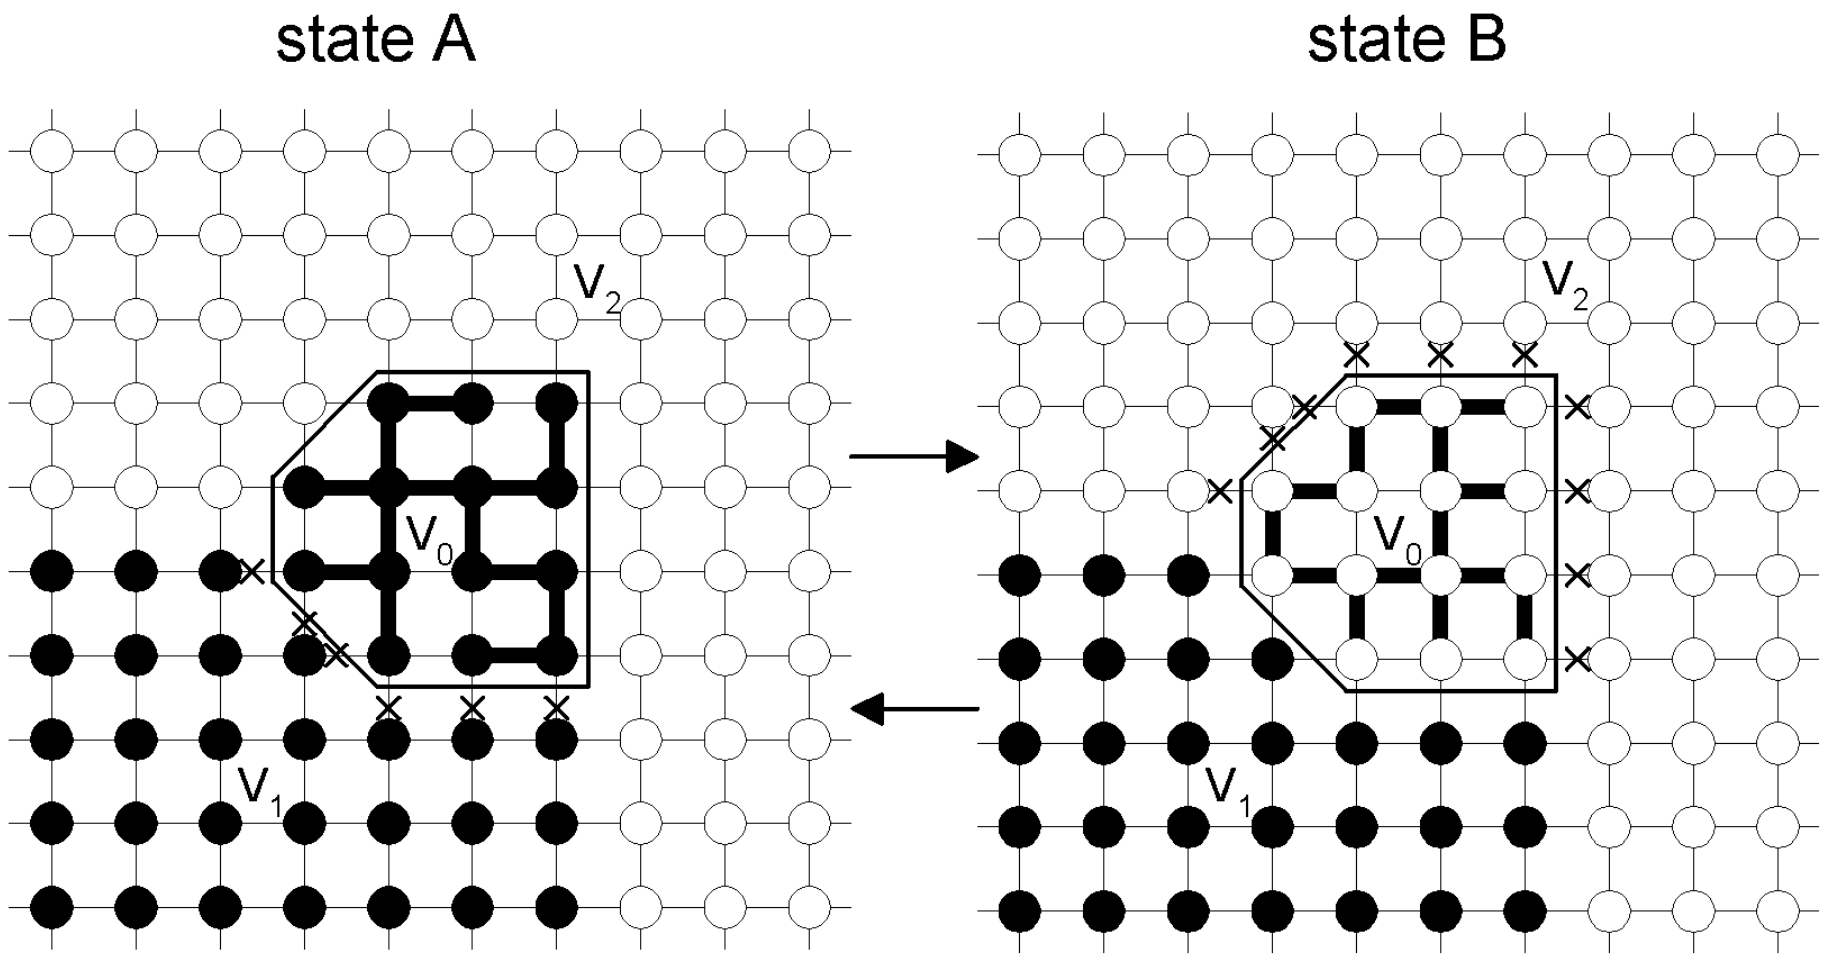
\includegraphics[width=0.6\textwidth]{figure/sw1.png}
    \caption{At each step, the SW algorithm flips a patch of vertices.}
    \label{fig:sw_onestep}
\end{figure}

As shown in Figure \ref{fig:sw_onestep}, suppose the current state is $A$ where $V_0$ is connected to $V_1$. The edges between $V_0$ and $V_1$ are turned off in the clustering step with the probability $e^{-\beta}$, from which we form a cut $C_{01}$ between $V_0$ and $V_1$ as $C_{01}=\{e=\epair{s,t},s\in V_0,t\in V_1\}$(as crosses in figure). Similarly, if the Markov chain is currently at state $B$, in order to achieve $A$, we also form a cut $C_{02}=\{e=\epair{s,t},s\in V_0,t\in V_2\}$. From the setting of Metroplis-Hastings, we need to compute the proposal probability $Q(A\to B)$ and $Q(B\to A)$, which is difficult but their ratio can be shown as 
\begin{equation}
\label{equ:proposal}
    \frac{Q(A\to B)}{Q(B\to A)}=\frac{e^{-\beta|C_{01}|}}{e^{-\beta|C_{02}|}}=e^{-\beta(|C_{01}|-|C_{02}|)}
\end{equation}
where $|\cdot|$ denotes the cardinality of a set. Remarkably, the ratio of the probability distribution is also decided by the size of the cuts because the probability distribution counts the number of connected edges.
\begin{equation}
    \frac{\pi(A)}{\pi(B)}=\frac{e^{-\beta|C_{01}|}}{e^{-\beta|C_{02}|}}=e^{-\beta(|C_{01}|-|C_{02}|)}
\end{equation}
Hence, the acceptance rate is given by
\begin{equation}
    \alpha(A\to B)=\min(1,\frac{Q(A\to B)\pi(B)}{Q(B\to A)\pi(A)})=1
\end{equation}
At low temperature, $\beta\propto 1/T$ and thus the SW flips large patches with acceptance rate $1$. Therefore, it can mix quickly even at critical temperatures. 

\begin{proof}(\textit{of Equation \ref{equ:proposal}})
Let $\mb{U}_A|(\mb{X}=A)$ and $\mb{U}_B|(\mb{X}=B)$ be realizations of $\mb{U}$ at state $A$ and state $B$. In the clustering step, we form two sets of connected components as $\mb{CP}(\mb{U}_A|\mb{X}=A)$ and $\mb{CP}(\mb{U}_B|\mb{X}=B)$. 

For $\mb{U}_A|(\mb{X}=A)$, following the Bernoulli probabilities, we divide the $\mb{U}_A$ into on and off edges as $\mb{U}_A=\mb{U}_{A,\text{on}}\cup \mb{U}_{A,\text{off}}$, where $\mb{U}_{A,\text{on}}=\{\mu_e\in \mb{U}_A:\mu_e=1\}$ and $\mb{U}_{A,\text{off}}=\{\mu_e\in \mb{U}_A:\mu_e=0\}$.

However, we are only interested in those $\mb{U}_A$ which are able to yield $V_0$. We collect all such $\mb{U}_A$ including $V_0$ given $A$ is a set, $\Omega(V_0|A)=\{\mb{U}_A: V_0\in \mb{CP}(\mb{U}_A|\mb{X}=A)\}$. To be concrete, in order to get $V_0$, all edges between $V_0$ and $V_1$ must be cut off. We denote the remaining off edges as $^{-}\mb{U}_{A,\text{off}}$ in a sense that $^{-}\mb{U}_{A,\text{off}}\cup C_{01}=\mb{U}_{A,\text{off}}$ for all $\mb{U}_A\in \Omega(V_0|A)$.

Similarly, we have $^{-}\mb{U}_{B,\text{off}}$ as $^{-}\mb{U}_{B,\text{off}}\cup C_{02}=\mb{U}_{B,\text{off}}$ for all $\mb{U}_A\in \Omega(V_0|B)$.

A key observation in this formulation is that there is a one-to-one mapping between $\Omega(V_0|A)$ and $\Omega(V_0|B)$ because we have a one-to-one mapping between $\mb{U}_A$ and $\mb{U}_B$ by setting $\mb{U}_{B,\text{on}}=\mb{U}_{A,\text{on}}$ and $\mb{U}_{B,\text{off}}=^{-}\mb{U}_{A,\text{off}}\cup C_{0,2}$.

That is, $\mb{U}_A$ and $\mb{U}_B$ only differ in the cuts and all these random variables inside the cuts are set as off. In other words, their connected components are the same $\mb{CP}(\mb{U}_A|\mb{X}=A)=\mb{CP}(\mb{U}_B|\mb{X}=B)$. Similarly, any $\mb{U}_B\in \Omega(V_0|B)$ has a one-to-one mapping to $\mb{U}_A\in \Omega(V_0|A)$.

Now suppose we choose $V_0\in \mb{CP}(\mb{U}_A|\mb{X}=A)$ randomly, its probability is
\[\mb{P}(V_0|A)=\sum_{\mb{U}_A\in \Omega(V_0|A)}\frac{1}{|\mb{CP}(\mb{U}_A|\mb{X}=A)|}\prod_{e\in \mb{U}_{A,\text{on}}}(1-e^{-\beta_e})\prod_{e\in ^{-}\mb{U}_{A,\text{off}}}e^{-\beta_e}\prod_{e\in C_{01}}e^{-\beta_e}\]

Similarly, the probability of choose $V_0$ in state $B$ is
\[\mb{P}(V_0|B)=\sum_{\mb{U}_B\in \Omega(V_0|B)}\frac{1}{|\mb{CP}(\mb{U}_B|\mb{X}=B)|}\prod_{e\in \mb{U}_{B,\text{on}}}(1-e^{-\beta_e})\prod_{e\in ^{-}\mb{U}_{B,\text{off}}}e^{-\beta_e}\prod_{e\in C_{02}}e^{-\beta_e}\]
In this way, we have
\[\frac{Q(A\to B)}{Q(B\to A)}=\frac{\mb{P}(V_0|A)}{\mb{P}(V_0|B)}=\frac{e^{-\beta|C_{01}|}}{e^{-\beta|C_{02}|}}=e^{-\beta(|C_{01}|-|C_{02}|)}\]
\end{proof}

\section{Hamilton Monte Carlo}
\kong{Just copy the original book for further understanding.}
\subsection{Hamilton Mechanics}
Hamiltonian Monte Carlo (HMC) is a powerful framework for sampling from high-dimensional continuous distributions. Langevin Monte Carlo (LMC) is a special case of HMC that is widely used in Deep Learning applications. Given an $n$-dimensional continuous density $P(X)$, the only requirement for implementing HMC is the differentiability of the energy $U(X) = -\log P(X)$. Like other MCMC methods (e.g. slice sampling, Swendsen-Wang cuts), HMC introduces auxiliary variables to facilitate movement in the original space. In HMC, the original variables represent \textit{position}, and the auxiliary variables represent \textit{momentum}. Each position dimension has a single corresponding momentum variable, so the joint space of the original and auxiliary variables has dimension $2n$, twice the size of the original space. Once the momentum variables are introduced, Hamilton’s Equations are used to simulate the time evolution of a physical system with potential energy $U$ . The properties of Hamilton’s Equations ensure that movement in the joint space preserves the distribution of $P$ in the original space.

Hamiltonian Mechanics was originally developed as an alternative but equivalent formulation of Lagrangian Mechanics, and both are equivalent to Newtonian Mechanics. In Hamiltonian Mechanics, the states of a physical system are represented by a pair of $n$- dimensional variables $q$ and $p$. The variable $q$ represents \textit{position} in the system, and $p$ represents \textit{momentum}. A joint state $(q, p)$ provides a complete description of the physical system at a single instant in time.

The evolution of a state $(q, p)$ over time is governed by a scalar-valued function $H(q, p)$ representing the energy of the system, and a pair of partial differential equations known as Hamilton’s Equations:
\begin{align*}
    \frac{dq}{dt}\aeq\frac{\partial H}{\partial p}\\
    \frac{dp}{dt}\aeq-\frac{\partial H}{\partial q}
\end{align*}
$H(q, p)$ is often referred to as the Hamiltonian of the system, and it remains constant as $(q,p)$ evolves over time.












\bibliography{references.bib}



%%%%%%%%%% Merge with supplemental materials %%%%%%%%%%
\clearpage
\begin{center}
\textbf{\Large Supplemental}
\end{center}


%%%%%%%%%% Prefix a "S" to all equations, figures, tables and reset the counter %%%%%%%%%%
\setcounter{equation}{0}
\setcounter{figure}{0}
\setcounter{table}{0}
\setcounter{page}{1}
\setcounter{section}{0}
\makeatletter
\renewcommand{\theequation}{S\arabic{equation}}
\renewcommand{\thefigure}{S\arabic{figure}}
%\renewcommand{\bibnumfmt}[1]{[S#1]}
%\renewcommand{\citenumfont}[1]{S#1}
%%%%%%%%%% Prefix a "S" to all equations, figures, tables and reset the counter %%%%%%%%%%
\subsection*{Formal Definition}
More details about this section can be found in \cite{Chung1960}. 

The basic building blocks of a probability theory can be formalized in the following:
\begin{enumerate}
    \item An abstract set $\Omega$, termed \textit{probability space} or \textit{sample space}, whose elements $\omega$ are called the \textit{elementary event} or \textit{sample point}.
    
    \item A Borel field $\mathfrak{F}$ of subsets of $\Omega$, termed \textit{measurable sets} or \textit{events}, in which $\Omega$ is also a member.
    
    \item An additive probability measure $P$ defined on $\mathfrak{F}$
\end{enumerate}
These together make the \textit{probability triple} $(\Omega, \mathfrak{F}, P)$ \todo{what's its physics analogy}. 



\textit{Why Borel field?}







% \textit{Random variable:}
% A real random variable is a single-valued function from a set $\Delta_0$ in $\mathfrak{F}$ to the closed real line $X = [-\infty, + \infty]$ such that for every real number $c$, the set of $\omega$ in $\Delta_0$ for which $x(\omega) \le c$ belongs to $\mathfrak{F}$. 



























































\subsection*{Microcanonical ensembles}

MCE focus on systems that are mechanically and adiabatically isolated from its environment ($\Delta E = W = Q = 0$). The general coordinates $\vec{x}$ is fixed, so that there is no work done i.e. $W = 0$; Internal energy  $E$ is also fixed since  $Q = 0\;\Rightarrow\;\Delta E = Q+W = 0$. This is the \textit{macrostate} given  $E, \vec{x}$, denoted by $M \equiv (E,\vec{x})$. \textit{The corresponding set of mixed microstates form the microcanonical ensemble}. 

A microstate in the phase space is labeled by $\mu$ i.e. phase space coordinate $\mu \equiv (x_1,p_1,\ldots,x_N,p_N)$, whose time evolution is governed by  $\mathcal{H}(\mu)$. In MCE, the Hamiltonian conserves the total energy of a given system, so all valid microstates are confined to the surface $\mathcal{H}(\mu) = E$. The central postulate of Statmech states that the equilibrium probability distribution is given by:
\begin{equation}
	P_{(E,\vec{x})} = \frac{1}{\Omega(E,\vec{x})}\cdot
	\begin{cases}
		1, & \text{for} \mathcal{H}(\mu) = E \\
		0, &\text{otherwise}
	\end{cases}
\end{equation}

\textbf{The zeroth law}

Consider two microcanonical systems (each with a large dof), their state in phase space are $\mu_1$ and  $\mu_2$ respectively. We allow them to exchange energy but not work. Remember these are systems modeled by MCE, so their state  $\mu_i$ is determined by internal energy $E_i$ and  $\vec{x}$ only. 

The combined system has energy:
\[
E = E_1 + E_2
.\] 
For this big system, (at any moment), its position in phase space is spanned by $\mu = \mu_1 \otimes \mu_2$. Therefore the Hamiltonian is described by:
\begin{equation}
	H(\mu_1 \otimes \mu_2) = H_1(\mu_1) + H_2(\mu_2)
\end{equation}
and
\begin{equation}
	P_E(\mu_1 \otimes \mu_2) = \frac{1}{\Omega(E)}\cdot
	\begin{cases}
		1 & \text{ for } H_1(\mu_1) + H_2(\mu_2) = E \\
		0 & \text{ otherwise}
	\end{cases}
\end{equation}
\textbf{Note: Here the Big system itself is viewed as a MCE!} Now we count how many states $\mu = \mu_1 \otimes \mu_2$ are possible. For each pair of  $\{E_1 \pm dE_1/2, E_2\pm dE_2/2\}$, there are  $\Omega_1(E_1)\times\Omega_2(E_2)$ states.  Therefore the total allowed states for the Big system is:
\begin{equation}
	\Omega(E) = \int dE_1 \Omega_1(E_1)\Omega_2(E-E_1)
\end{equation}
we can write $\Omega$ as  $\Omega = \exp{\log(\Omega)} = \exp{S/k_B}$, so:
 \begin{equation}
	 \Omega(E) = \int dE_1 \exp{\frac{S_1(E_1)+S_2(E-E_1)}{k_B}}
\end{equation}
According to (3), all states are equal weighted, therefore the energy that produces largest $\Omega(E)$ is the equilibrium energy we are looking for. Since the integrand is exponentially large, we expect the mean contribution is from the peak defined at $E_1^*$, so that  $S_1 + S_2$ is maximized, thus the total entropy is maximized:
 \begin{equation}
	 S(E) = k_B \log\Omega(E) \simeq S_1(E_1^*) + S_2(E_2^*) \text{ is maximized}
\end{equation}
Now we find $E_1$ that maximize  $S_1 + S_2$:
\begin{equation}
\begin{split}
	\frac{\partial }{\partial E_1}&\Bigl( S_1(E_1) + S_2(E-E_1) \Bigr)
	 = \frac{\partial S_1}{\partial E_1} + \frac{\partial S_2(E-E_1)}{\partial E_1}\\
				      &=\frac{\partial S_1}{\partial E_1} - \frac{\partial S_2}{\partial E_2} = 0
\end{split}
\end{equation}
therefore:
\begin{equation}
	\frac{\partial S_1}{\partial E_1} = \frac{\partial S_2}{\partial E_2}
\end{equation}
which must be satisfied when the joint system reach the equilibrium! It is consistent with zeroth law, that systems in equilibrium has equal temperautre:
\begin{equation}
	\frac{\partial S}{\partial E}\Big|_{\textbf{x}} = \frac{1}{T}
\end{equation}
note they are evaluated at their own fixed  \textbf{x}.



\subsection*{Canonical ensembles}

\clearpage
\begin{center}
\textbf{\Large The story of sampling}
\end{center}
This part, I will recap the history of sampling from the posterior distribution, which is a unique chance to grasp the main idea of sampling in statistics. Thanks S. Feng.

In history, with the power of Central Limit Theorem, we can use a single point estimate for a parameter and its standard error. (\kong{CLT talks about asymptotic normality of a distribution, but why we call it a single point estimation and does it has anything to do with estimate of sample mean?}) However, in the view of Bayesian analysis, we seek to summarize the entire posterior distribution. The key difference lies in that here Bayesian tends to use entire posterior distribution rather than the mode of likelihood function and standard errors. In the same way, if we are able to summarize the entire posterior distribution for a parameter, there is no need to rely on asymptotic arguments about the normality of the distribution: It can be directly assessed. 









\end{document}

% \begin{table}
%  \caption{Sample table title}
%   \centering
%   \begin{tabular}{lll}
%     \toprule
%     \multicolumn{2}{c}{Part}                   \\
%     \cmidrule(r){1-2}
%     Name     & Description     & Size ($\mu$m) \\
%     \midrule
%     Dendrite & Input terminal  & $\sim$100     \\
%     Axon     & Output terminal & $\sim$10      \\
%     Soma     & Cell body       & up to $10^6$  \\
%     \bottomrule
%   \end{tabular}
%   \label{tab:table}
% \end{table}